\clearpage
\subsection{Diffusion model}


The diffusion model was trained on a subset of the American Mineralogist dataset using paired synthetic and measured X-ray diffraction (XRD) patterns.
To evaluate the proposed denoising architecture, we trained an improved 1D diffusion-based U-Net on a dataset comprising 13\,325 paired synthetic and real diffraction patterns. Each sample consists of a synthetic XRD signal (\texttt{synth\_xrd}), a corresponding experimental measurement (\texttt{real\_xrd}), and a precomputed fast dynamic time warping (FastDTW) distance (\texttt{fast\_dtw\_distance}). This distance was used as a proxy for structural or noise-level divergence and served as a scalar conditioning variable (hereafter referred to as ``temperature'') during training. The data was randomly split into 70\% training, 15\% validation, and 15\% test sets, with care taken to maintain a balanced temperature distribution across subsets.\\

The model employs a modified 1D U-Net architecture combined with a forward diffusion process. The diffusion process adds Gaussian noise along with domain-specific augmentations. The temperature variable is used to condition the model based on the similarity between synthetic and real samples. This conditioning is implemented via a feedforward neural network and allows the model to learn to denoise patterns with varying noise levels. In practice, the temperature can be interpreted as a user-controllable parameter to adjust the degree of denoising. The architecture is designed to be modular and scalable: the number of downsampling and upsampling blocks can be increased or reduced based on the available hardware. For this study, to limit memory usage, we instantiated the model with a hidden dimensionality of 16 channels and two downsampling levels.\\

The forward diffusion process follows a cosine noise schedule over 1\,000 timesteps. A linear schedule was also tested but yielded less stable results. In addition to noise, the forward process includes domain-aware augmentations such as peak broadening (using a Gaussian kernel derived from the Scherrer equation), intensity perturbation, and random peak shifting or removal. These augmentations are scaled by timestep to simulate increasingly severe physical and instrumental noise.\\

Training was conducted for 100 epochs using the AdamW optimizer with a learning rate of $1 \times 10^{-4}$, cosine annealing learning rate scheduling, and gradient clipping ($\text{max\_norm} = 1.0$). The loss function was a weighted sum of two components:\\

\begin{itemize}
    \item \textbf{Diffusion Loss:} Mean squared error (MSE) between the predicted and true Gaussian noise in the forward process.
    \item \textbf{Reconstruction Loss:} MSE between the denoised output from real patterns and the corresponding synthetic target.
\end{itemize}

Since real XRD patterns often contain more than just sharp peaks, we initially guide the model using primarily augmented synthetic data. As training progresses, emphasis shifts toward accurately reconstructing measured samples. The experimental data used for validation was high-quality and lacked significant peak broadening, so a phased training strategy was adopted to improve generalisation. Training was divided into three phases. Initially, diffusion loss was prioritised to help the model learn the generative process. In later phases, more weight was given to reconstructing realistic patterns. Table~\ref{tab:loss-weights} summarises the loss weights and timestep schedule used in each phase.\\

\begin{table}[!h]
\centering
\caption{Loss weighting and timestep schedule by training phase.}
\label{tab:loss-weights}
\begin{tabular}{|c|c|c|c|c|}
\hline
\textbf{Phase} & \textbf{Epoch Range} & $\boldsymbol{\lambda_{\text{diff}}}$ & $\boldsymbol{\lambda_{\text{recon}}}$ & \textbf{Max Timestep} \\
\hline
1 & 0--32  & 0.8 & 0.2 & 500 \\
2 & 33--65 & 0.5 & 0.5 & 750 \\
3 & 66--99 & 0.1 & 0.9 & 1000 \\
\hline
\end{tabular}
\end{table}



\subsubsection{Replication of measured patterns}

To assess whether the diffusion model can replicate measured signals given only the ideal Rietveld-derived input, we passed each test-set synthetic pattern through the trained model at $t{=}0$ (i.e.\ direct ideal-to-realistic mapping) and compared the output against the corresponding laboratory measurement.
Figure~\ref{fig:overlay_comparison} presents four representative overlay plots, selected at the 10th, 35th, 65th, and 90th percentiles of the DTW distance distribution.
The percentile selection ensures that we examine performance across both easy cases, where the synthetic and real patterns are already similar, and difficult cases where significant instrumental and structural divergence exists.

At low DTW distances the model output closely traces the measured curve, preserving both peak positions and relative intensities. As the DTW distance increases, the task becomes harder and the model must account for larger discrepancies in peak broadening and background shape. Even at the 90th percentile the principal Bragg reflections are recovered, although minor deviations in the background region and low-intensity shoulders become visible. Overall, the overlays confirm that the model has learned a meaningful mapping from idealised to experimentally realistic patterns.

\begin{figure}[htbp]
    \centering
    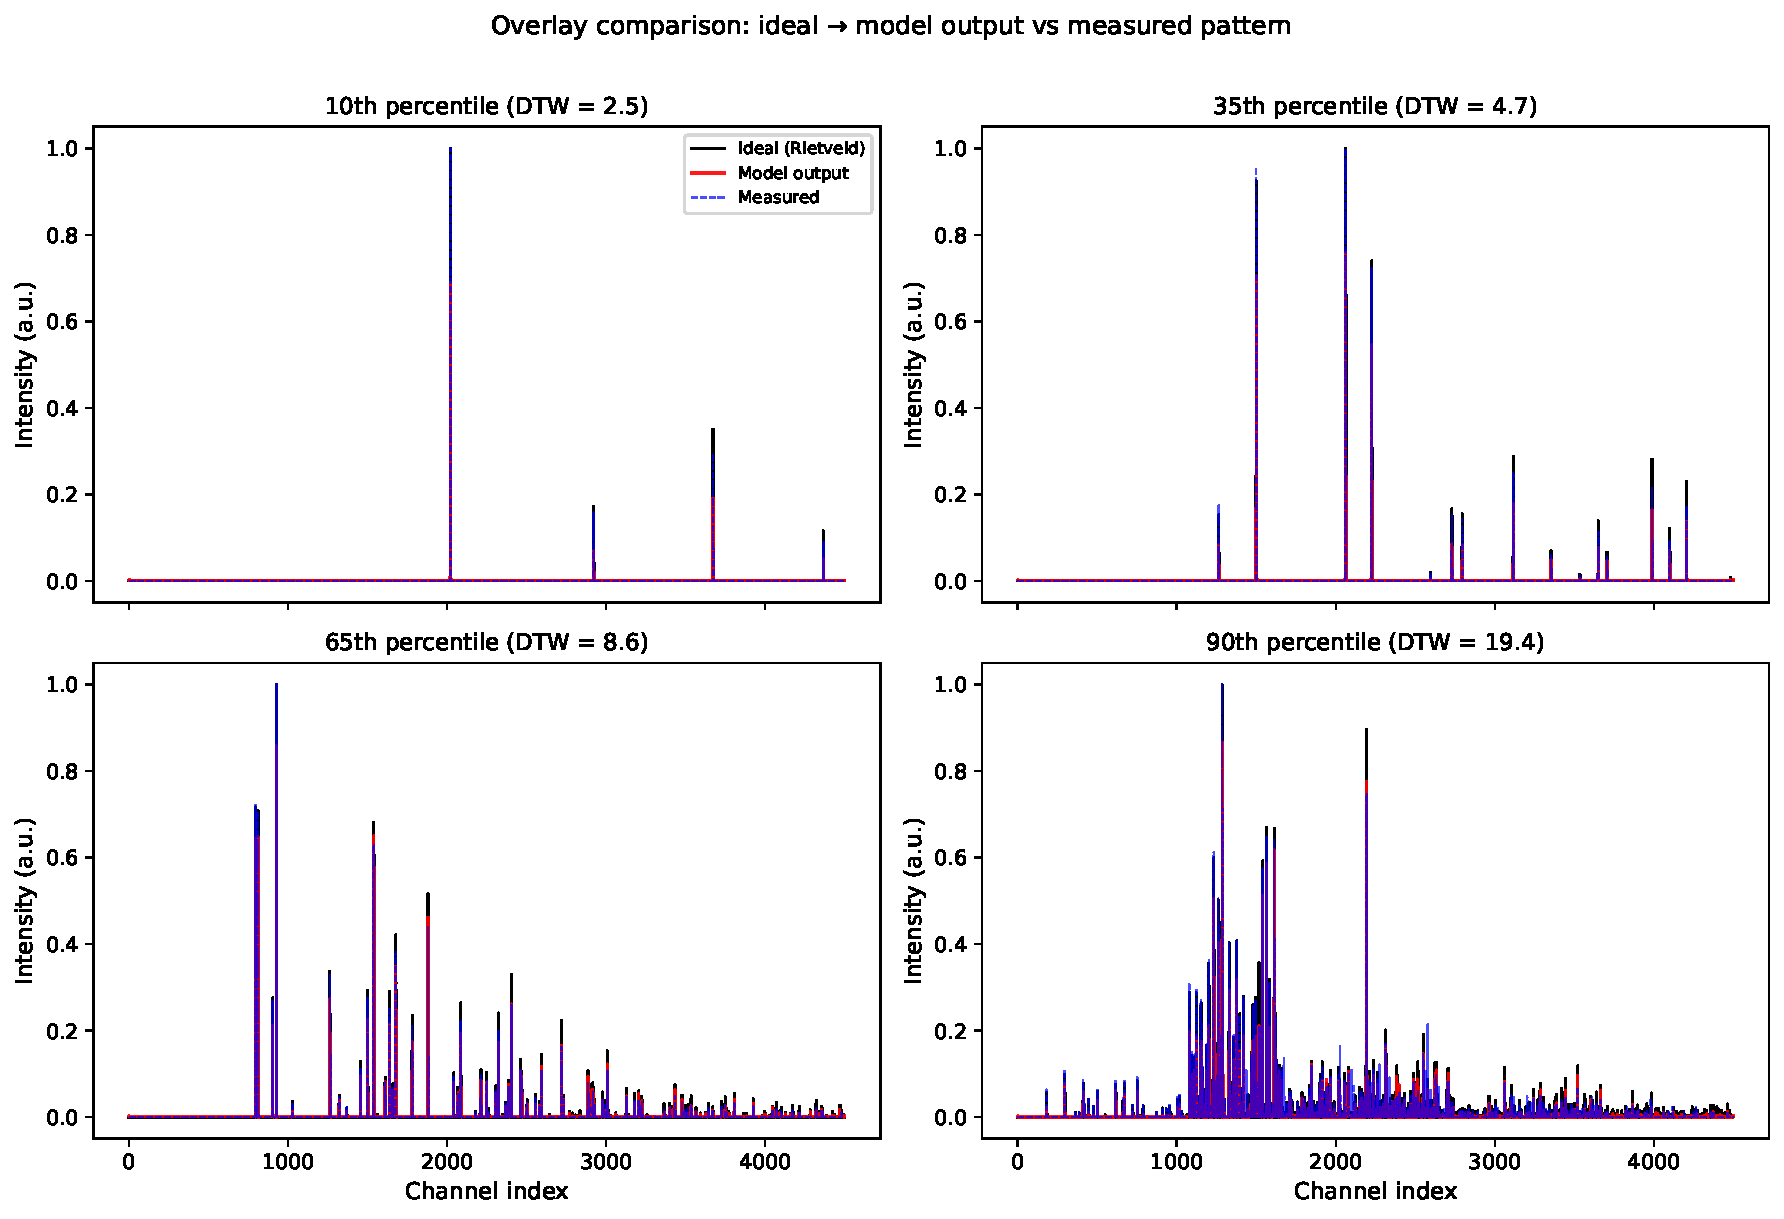
\includegraphics[width=0.95\linewidth]{figures/overlay_comparison.pdf}
    \caption{Overlay comparison of ideal (Rietveld) input, model output at $t{=}0$, and measured pattern for four test samples at increasing DTW distance (10th, 35th, 65th, 90th percentile).}
    \label{fig:overlay_comparison}
\end{figure}


\subsubsection{Stochastic variation analysis}

A diffusion model is inherently stochastic: different random noise draws in the forward process yield different denoised outputs even for the same input.
To quantify this variation we fixed a single ideal pattern (35th DTW percentile) and applied the forward process at $t{=}50$ with $N{=}1\,000$ independent noise realisations, denoising each via Equation~\ref{eq:denoise}.

Figure~\ref{fig:stochasticity_spread} displays the mean output spectrum together with its $\pm 1\sigma$ band, overlaid with the ideal input and the actual measured pattern.
The shaded band is narrow across most of the pattern, indicating that the model produces tightly clustered outputs despite the stochastic process. The measured pattern falls within or very close to this band, suggesting that the model's output distribution encompasses the real measurement.

Figure~\ref{fig:mae_histogram} shows the distribution of mean absolute error (MAE) between each of the 1\,000 stochastic outputs and the ideal input.
The histogram is concentrated around its mean, confirming that the forward-diffusion noise at $t{=}50$ induces only a small, controlled perturbation that the model denoises consistently.

We further examined whether the stochastic variation affects the crystallographic peak positions recovered by the model, since peak positions encode the lattice parameters and are the primary observable used for phase identification.
For each of the $N{=}1\,000$ runs we located the nearest local maximum within $\pm$15 channels of every reference peak detected on the mean spectrum, then computed the coefficient of variation (CV) of each peak's position.
Figure~\ref{fig:cv_peak_positions} shows that all detected peaks have CV well below the 5\,\% stability threshold.
This confirms that, although the model output varies stochastically in amplitude and background detail, the positions of crystallographic reflections remain stable.

\begin{figure}[htbp]
    \centering
    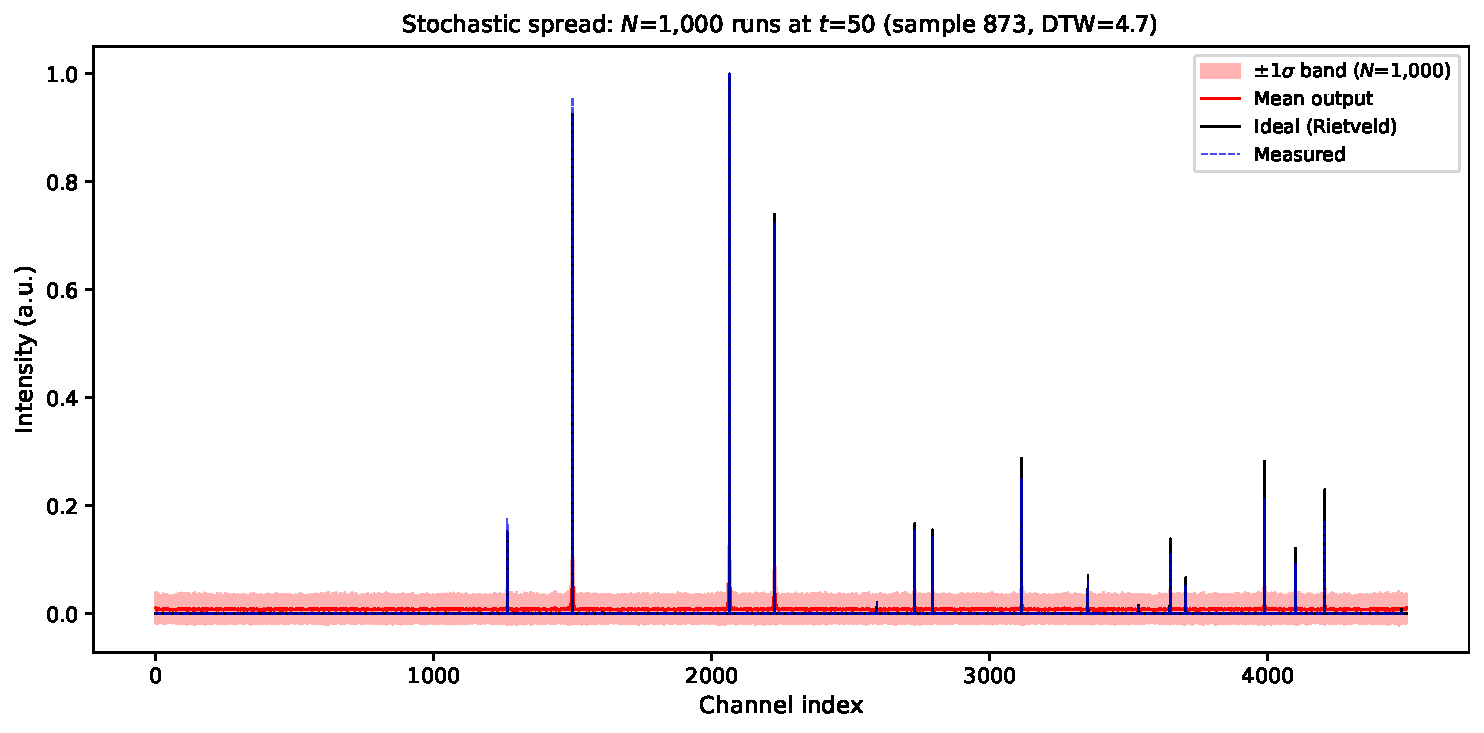
\includegraphics[width=0.85\linewidth]{figures/stochasticity_spread.pdf}
    \caption{Stochastic spread for a single ideal input at $t{=}50$ across $N{=}1\,000$ independent noise draws. The red band shows $\pm 1\sigma$ around the mean output; the blue dashed line is the actual measured pattern.}
    \label{fig:stochasticity_spread}
\end{figure}

\begin{figure}[htbp]
    \centering
    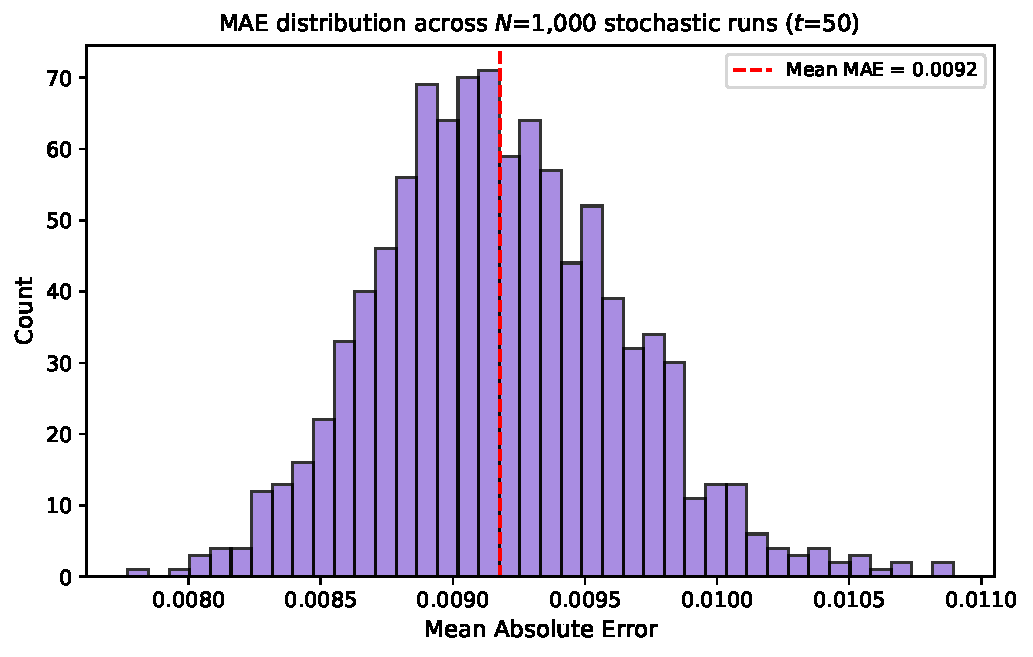
\includegraphics[width=0.7\linewidth]{figures/mae_histogram.pdf}
    \caption{Distribution of mean absolute error across $N{=}1\,000$ stochastic runs at $t{=}50$, each compared to the ideal input.}
    \label{fig:mae_histogram}
\end{figure}

\begin{figure}[htbp]
    \centering
    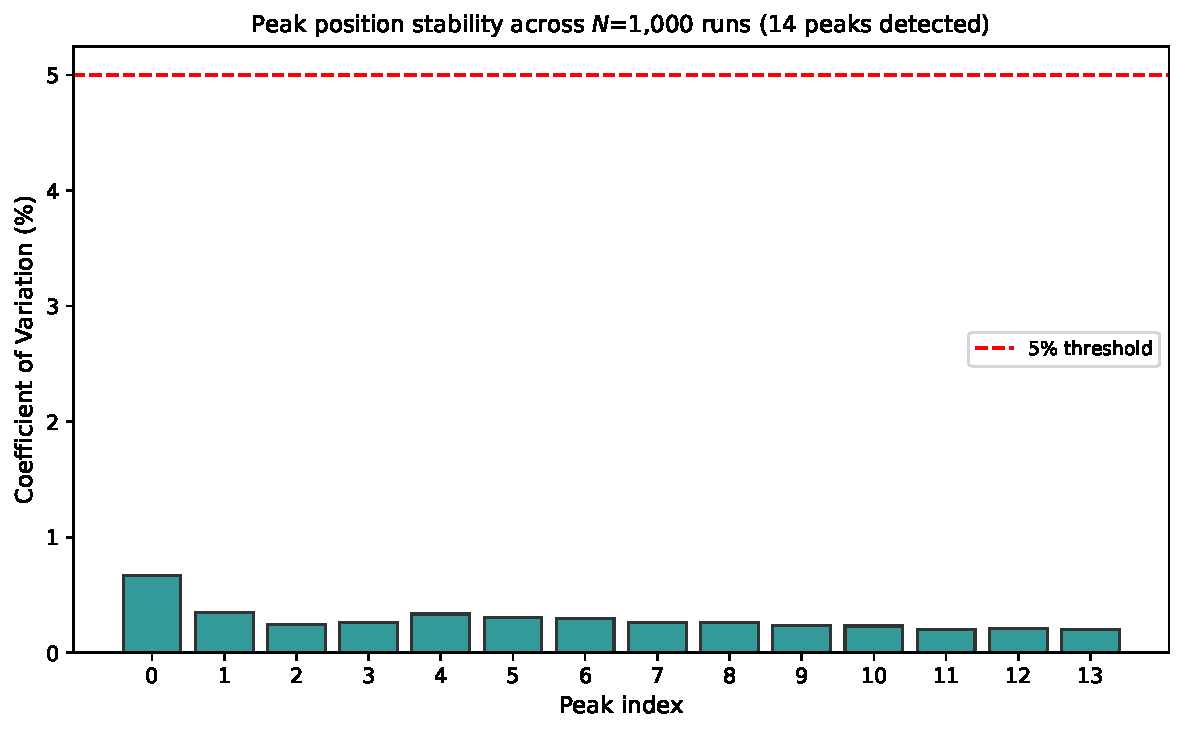
\includegraphics[width=0.85\linewidth]{figures/cv_peak_positions.pdf}
    \caption{Coefficient of variation (\%) of each detected peak position across $N{=}1\,000$ stochastic runs. The red dashed line marks the 5\,\% stability threshold; all peaks fall well below it.}
    \label{fig:cv_peak_positions}
\end{figure}


\subsubsection{Effect of noise level on denoising}

To visualise how the noise-level parameter controls the degree of transformation, we passed the same ideal pattern through the forward process at timesteps $t \in \{0, 50, 100, 200, 500, 900\}$ and denoised each.
Figure~\ref{fig:denoising_waterfall} presents the result as a heatmap where each row corresponds to a different noise level.
At $t{=}0$ the output is essentially a direct ideal-to-realistic mapping with no added stochasticity. As $t$ increases the model must denoise progressively larger perturbations, and the output gradually diverges from the clean input.
For moderate timesteps ($t \leq 200$) the pattern remains recognisable and the principal peaks are preserved. At higher timesteps ($t{=}500$ and $t{=}900$) the model still attempts to recover the clean signal, but increasing noise magnitude leads to visible artefacts, particularly in the background region.
These results confirm that timestep selection offers a useful dial for controlling the strength of the stochastic augmentation.

\begin{figure}[htbp]
    \centering
    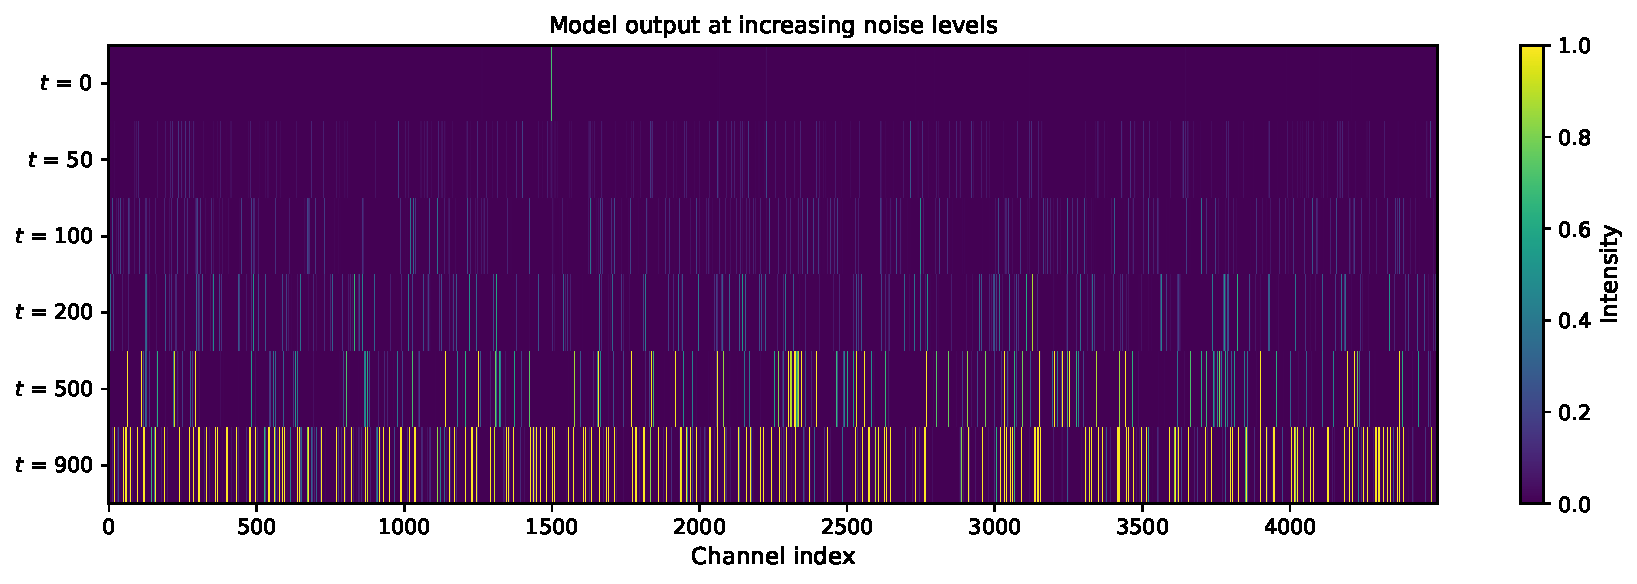
\includegraphics[width=0.95\linewidth]{figures/denoising_waterfall.pdf}
    \caption{Heatmap of denoised output at increasing noise levels ($t = 0, 50, 100, 200, 500, 900$) for a single ideal input. Lower rows correspond to stronger noise in the forward process.}
    \label{fig:denoising_waterfall}
\end{figure}


\subsubsection{Quantitative evaluation on the test set}

We evaluated the full test set ($n = 2\,000$ held-out samples) by passing every synthetic pattern through the model at $t{=}0$ and comparing the output against the corresponding measured pattern.
Table~\ref{tab:quant-metrics} summarises the results.

\begin{table}[htbp]
\centering
\caption{Quantitative comparison of model output ($t{=}0$) against measured patterns on the held-out test set.}
\label{tab:quant-metrics}
\begin{tabular}{|l|c|}
\hline
\textbf{Metric} & \textbf{Mean $\pm$ Std} \\
\hline
RMSE                        & 0.0103 $\pm$ 0.0059 \\
Pearson correlation ($r$)   & 0.872 $\pm$ 0.185 \\
Normalised cross-correlation & 0.872 $\pm$ 0.185 \\
\hline
\end{tabular}
\end{table}

Figure~\ref{fig:quantitative_metrics} shows the per-sample distributions of RMSE and Pearson correlation across the test set.
The RMSE histogram is concentrated at low values, indicating that model outputs are quantitatively close to the measured patterns for the majority of samples.
The Pearson correlation distribution is skewed toward high positive values, confirming strong linear agreement between predicted and measured intensities.
Together these metrics demonstrate that the model does not merely reproduce the correct peak positions but also captures the relative intensities and background shape with high fidelity.

\begin{figure}[htbp]
    \centering
    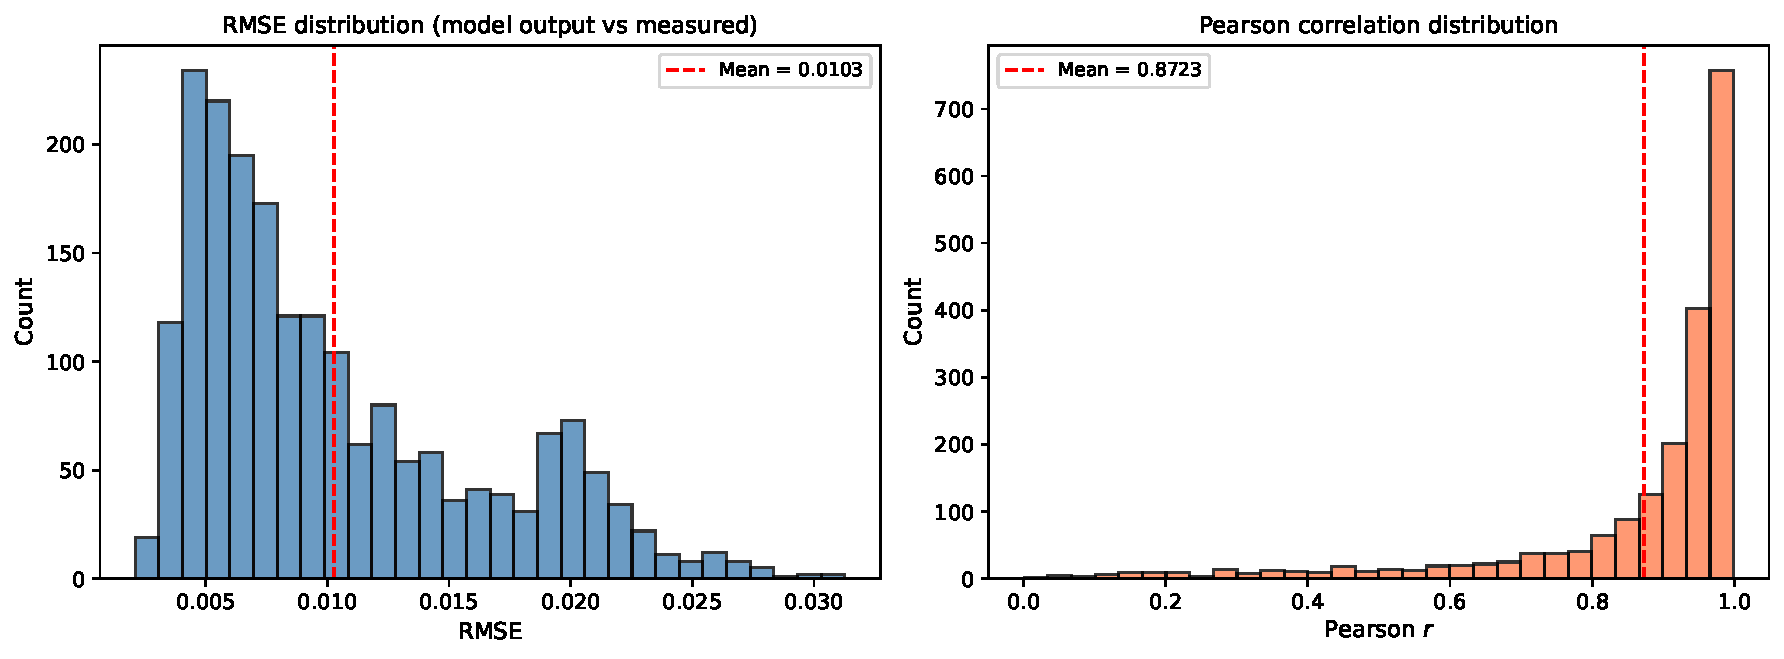
\includegraphics[width=0.95\linewidth]{figures/quantitative_metrics.pdf}
    \caption{Per-sample distributions of RMSE (left) and Pearson correlation (right) between model output at $t{=}0$ and measured patterns across the full test set. Red dashed lines indicate the mean.}
    \label{fig:quantitative_metrics}
\end{figure}


\subsubsection{Training convergence}

Figure~\ref{fig:training_history} shows the training and validation loss curves over 100 epochs.
Both losses decrease sharply during the first phase (epochs 0--32, dominated by diffusion loss) and continue to decline more gradually through the second phase (epochs 33--65, balanced weighting).
In the third phase (epochs 66--99), where reconstruction loss carries $\lambda_{\text{recon}} = 0.9$, the validation loss stabilises, indicating convergence without over-fitting.
The loss-component breakdown confirms that the diffusion term accounts for most of the early improvement, while later gains are driven by the reconstruction objective as intended by the phased weighting strategy.

\begin{figure}[htbp]
    \centering
    \includegraphics[width=0.9\linewidth]{Pictures/training_history.png}
    \caption{Training and validation loss over 100 epochs with phase transitions at epochs 33 and 67. Upper panel: combined loss; lower panel: individual diffusion and reconstruction loss components. The phased weighting schedule (Table~\ref{tab:loss-weights}) shifts emphasis from noise prediction to pattern reconstruction across the three phases.}
    \label{fig:training_history}
\end{figure}
